% folarrow-ja.tex：folarrowパッケージの説明書
% 組み方：uplatex folarrow-ja && dvipdfmx folarrow-ja
% （xy-picの例を含むのでupLaTeX＋dvipdfmxで組む．TeX Live 2025と2026のLuaLaTeXでは
%   xy-pic自体がxypdfのエラーになる）
\documentclass[dvipdfmx,paper=a4]{jlreq}
\usepackage{amsmath,amscd}
\usepackage[all]{xy}
\usepackage{tikz-cd}
\usepackage{folarrow}
\usepackage{fancyvrb}
\usepackage{graphicx}
\usepackage{longtable}
\usepackage{url}
\title{folarrowパッケージ\\\large 葉層束の射影を表す3本線入り矢印}
\author{木枝祐介}
\date{2026年10月10日　v20261010.0}
\newcommand\pkg[1]{\textsf{#1}}
\newcommand\cs[1]{\texttt{\textbackslash#1}}
\newcommand\file[1]{\texttt{#1}}
\fvset{frame=single,framesep=3mm,fontsize=\small}
\begin{document}
\maketitle

\noindent 英語版の説明書は\file{folarrow-en.pdf}である．

\section{概要}

ファイバー束を図式で書くとき，射影を縦向きの矢印で描く．
\[
\begin{CD}
V @>>> E\\
@. @VV{\pi}V\\
@. M
\end{CD}
\]
葉層束では，この射影の矢印の軸に3本の斜線を入れて表すことがある．
\[
\begin{CD}
V @>>> E\\
@. @FVV{\pi}V\\
@. M
\end{CD}
\]
\pkg{folarrow}は，この矢印を\pkg{amscd}，\pkg{xy-pic}，\pkg{tikz-cd}の図式と，本文の数式で
使えるようにする．

矢印そのものは各パッケージの通常の矢印をそのまま使い，軸の中ほどに3本の斜線を重ねる．
斜線は\pkg{pict2e}（\pkg{tikz-cd}ではPGF）で描くので，フォントを追加する必要はない．
斜線の長さと線の太さは，その場の数式フォントの大きさ（文字サイズ・添字のスタイル）に合わせて決まる．

\section{読み込み}

\begin{Verbatim}
\usepackage{amscd}      % 使うものだけ
\usepackage[all]{xy}
\usepackage{tikz-cd}
\usepackage{folarrow}
\end{Verbatim}
\pkg{amscd}，\pkg{xy-pic}，\pkg{tikz-cd}は\pkg{folarrow}の前後どちらで読み込んでもよい
（対応の設定は\verb|\begin{document}|で行う）．

\subsection{簡易版（\texttt{lite}オプション）}\label{sec:lite}
\begin{Verbatim}
\usepackage[lite]{folarrow}
\end{Verbatim}
\verb|lite|を付けると，ほかのファイル（Luaのモジュール，実測データ，矢印のフォント）を使わず，
すべての矢印を描いて組む簡易版になる（簡易版だけの説明書\file{folarrow-lite-ja.pdf}もある）．
矢印のフォントをPDFに埋め込まずに組みたいときなどに使う．付けなければ（既定）これまでどおりである．
\begin{itemize}
\item \file{folarrow.sty}以外のファイルは，インストールされていても一切使わない．使わないのは，
  Luaのモジュール\file{folarrow.lua}，実測データ\file{folarrow-fonts.def}，矢印のフォントの表
  \file{folarrow-glyphs.def}と\file{folarrow-otf.def}，矢印のフォントとマップファイルである．
\item 本文用の矢印も含め，すべての矢印を描いて組む（\ref{sec:glyphs}節のフォントは使わず，
  \verb|glyphs|は常にfalseになる）．組版の結果は矢印と3本線の重ね合わせなので，PDFからテキストとして
  取り出すと元の矢印の文字（\verb|\foldownarrow|では区切り記号の部品）になる．
\item 矢頭の幅と線の太さ（\ref{sec:metrics}節）は，Xe\LaTeX{}でOpenTypeの数式フォントを使うときは
  グリフの外接矩形から読み（\verb|\XeTeXglyphbounds|を使う），それ以外（pdf\LaTeX，up\LaTeX，Lua\LaTeX{}）では
  フォントの寸法から推定する．
\item 実測データを使わないので，3本線は矢印の箱の中央に置き（字面の中心とのずれを補正しない），
  3本線の端はつねに切りっぱなしにする．10\,ptのComputer Modern，\pkg{newtxmath}，\pkg{newpxmath}，
  \pkg{txfonts}の本文用の矢印では，3本線の中央からのずれは矢印の向きに最大0.3\,pt，直交方向に0.03\,pt
  だった（既定では0.015\,pt以下）．書体によってはもっと大きくずれ，幅や太さも実測値と違うことがある．
\item Pennstander Mathの縦向きの矢印を回して組む対処（\ref{sec:glyphs}節）も行わない．
\item \verb|lite|はパッケージの読み込み時にだけ指定できる（\verb|\folarrowsetup|では変えられない）．
\end{itemize}

\section{amscd}

通常の矢印の指定\verb|@>>>|，\verb|@<<<|，\verb|@VVV|，\verb|@AAA|の\verb|@|の直後に
\verb|F|を付けると，斜線入りになる．ラベルの書き方は通常の矢印と同じである．
\begin{Verbatim}
\begin{CD}
V @>>> E @F>f>> E'\\
@VVV @FV{\pi}VV @FAA{\pi'}A\\
M @= M @F<<g< M
\end{CD}
\end{Verbatim}
\[
\begin{CD}
V @>>> E @F>f>> E'\\
@VVV @FV{\pi}VV @FAA{\pi'}A\\
M @= M @F<<g< M
\end{CD}
\]

\section{xy-pic}

矢印の途中に置く方向付きの物体\verb|fol|を用意した．\verb/\ar[d]|@{fol}/のように，
\verb/|/（矢印上のラベル）として置く．大きさ0の物体なので矢印は途切れない．
斜線の向きは矢印の向きから自動で決まり，斜めの矢印にも使える．
\begin{Verbatim}
\xymatrix{
V \ar[r] & E \ar[d]|@{fol}^{\folpad{\pi}} \\
         & M }
\end{Verbatim}
\[
\xymatrix{
V \ar[r] & E \ar[d]|@{fol}^{\folpad{\pi}} \\
         & M }
\qquad
\xymatrix{
E \ar[r]|@{fol} & B \ar[d]|@{fol} \ar[dl]|@{fol} \\
M \ar[u]|@{fol} & N \ar[l]|@{fol} }
\]

矢印のラベルは斜線の位置に来るので，そのままでは斜線にかかることがある．
ラベルを\verb|\folpad|で囲むと，四方に斜線の半分の長さの余白が付いて斜線を避ける．
\begin{Verbatim}
\ar[d]|@{fol}^{\folpad{\pi}}
\end{Verbatim}

\section{tikz-cd}

矢印のオプションに\verb|foliated|を加える．
\begin{Verbatim}
\begin{tikzcd}
V \arrow[r] & E \arrow[d, foliated, "\pi"] \\
            & M
\end{tikzcd}
\end{Verbatim}
\[
\begin{tikzcd}
V \arrow[r] & E \arrow[d, foliated, "\pi"] \\
            & M
\end{tikzcd}
\qquad
\begin{tikzcd}
E \arrow[r, foliated] & B \arrow[d, foliated] \arrow[dl, foliated] \\
M \arrow[u, foliated] & N \arrow[l, foliated]
\end{tikzcd}
\]
\verb|foliated|は\verb|decorations.markings|ライブラリーを使う（\pkg{folarrow}が読み込む）．
\verb|foliated|を付けた矢印では，ラベルが斜線にかからないよう，ラベルの余白（\verb|inner sep|）を
斜線の半分の長さだけ増やす．

\section{本文の数式}

\begin{center}
\renewcommand\arraystretch{1.5}
\begin{tabular}{ll}
\verb|\folrightarrow| & $E\folrightarrow M$\\
\verb|\folleftarrow| & $M\folleftarrow E$\\
\verb|\foldownarrow| & $E\foldownarrow M$\\
\verb|\foluparrow| & $M\foluparrow E$\\
\verb|\xfolrightarrow[下]{上}| & $E\xfolrightarrow{\pi}M$，\ $E\xfolrightarrow[\text{proj}]{\pi}M$\\
\verb|\xfolleftarrow[下]{上}| & $M\xfolleftarrow{\pi}E$
\end{tabular}
\end{center}
\begin{itemize}
\item いずれも関係記号（\verb|\mathrel|）で，添字の中でも使える：$A_{E\folrightarrow M}$．
\item 土台の矢印：\verb|\folrightarrow|は\verb|\longrightarrow|，\\
  \verb|\folleftarrow|は\verb|\longleftarrow|．
\item \verb|\xfolrightarrow|と\verb|\xfolleftarrow|は，\pkg{amsmath}の\verb|\xrightarrow|と同じく
  上下のラベルに合わせて伸びる．ただし\verb|\longrightarrow|より短くはならない．
\end{itemize}

\subsection{本文用の矢印のフォント}\label{sec:glyphs}
\verb|\folrightarrow|，\verb|\folleftarrow|，\verb|\foldownarrow|，\verb|\foluparrow|の4つは，
次の数式フォントでは，3本線まで含めて1つの字形になったType~1フォントで組む．
\begin{center}
\begin{tabular}{lll}
数式フォント & 記号フォント & 矢印のフォント\\\hline
Computer Modern（既定） & \file{cmsy5}〜\file{cmsy10} & \file{folcm5}〜\file{folcm10}\\
Latin Modern（\pkg{lmodern}） & \file{lmsy5}〜\file{lmsy10} & \file{follm5}〜\file{follm10}\\
\pkg{newtxmath} & \file{ntxsy}，\file{ntxsy7}，\file{ntxsy5} & \file{folntx}，\file{folntx7}，\file{folntx5}\\
\pkg{txfonts} & \file{txsy} & \file{foltx}\\
\pkg{newpxmath} & \file{zplsy} & \file{folzpl}\\
\pkg{pxfonts} & \file{pxsy} & \file{folpx}\\\hline
Computer Modern（ボールド） & \file{cmbsy5}〜\file{cmbsy10} & \file{folcmb5}〜\file{folcmb10}\\
Latin Modern（ボールド） & \file{lmbsy5}，\file{lmbsy7}，\file{lmbsy10} & \file{follmb5}，\file{follmb7}，\file{follmb10}\\
\pkg{newtxmath}（ボールド） & \file{ntxbsy}，\file{ntxbsy7}，\file{ntxbsy5} & \file{folntxb}，\file{folntxb7}，\file{folntxb5}\\
\pkg{txfonts}（ボールド） & \file{txbsy} & \file{foltxb}\\
\pkg{newpxmath}（ボールド） & \file{zplbsy} & \file{folzplb}\\
\pkg{pxfonts}（ボールド） & \file{pxbsy} & \file{folpxb}
\end{tabular}
\end{center}
\begin{itemize}
\item 字形は，記号フォントのマイナス記号と→（\verb|\longrightarrow|と同じ組み方）の輪郭に，
  3本線の輪郭を加えたものである．←はマイナス記号と←，↓と↑は→の字形を回したもので，
  数式の軸に中心を合わせる．3本線の長さ・間隔・傾き・太さ・端の形は，描く場合の既定値と同じ規則で，
  元の字形の輪郭から求めた．3本線の中心は矢印の字面の中央にある．
\item 組版の結果はフォントの1文字なので，PDFからテキストとして取り出すと→，←，↓，↑
  （U+2192，U+2190，U+2193，U+2191）になる．
\item フォントは記号フォントと同じ大きさで読むので，添字の中や\verb|\large|などでも，
  その大きさの記号フォントに対応する字形になる．
\item 形のキー（\ref{sec:shape}節）が既定値でないとき，\verb|glyphs=false|のとき，
  上の表にも次のOpenTypeの数式フォントの表にもない数式フォントでは，これまでどおり
  矢印に3本線を描いて組む．このとき↓↑の土台は，記号フォントのquadの1.25倍の高さの区切り記号である．
\item 伸びる矢印（\verb|\xfolrightarrow|など）と図式の矢印は，長さが変わるので常に描く．
\end{itemize}
\paragraph{OpenTypeの数式フォント}
Lua\LaTeX{}とXe\LaTeX{}で\pkg{unicode-math}を使うときは，次の49書体に対応するOTF
（\file{folu-〈略号〉.otf}）で組む．
\begin{quote}\small
Latin Modern Math，New Computer Modern Math（Regular，Book，Bold），New Computer Modern Sans Math，
STIX Two Math，STIX Math，XITS Math（Regular，Bold），\TeX{} Gyre Termes／Pagella／Bonum／Schola／DejaVu Math，
Libertinus Math，Fira Math，Asana Math，Erewhon Math（Regular，Bold），
KpMath（Regular，Light，Semibold，Bold，Sans，SansBold），GFS Neohellenic Math，IBM Plex Math，
Arsenal Math（Sans，SansBold），Concrete Math（Regular，Bold），Euler Math，Garamond Math，
Lete Sans Math（Regular，Bold），Luciole Math（Regular，Bold），Old Standard Math，
XCharter Math（Regular，Bold），Pennstander Math（Thin〜Blackの9つ）
\end{quote}
\begin{itemize}
\item XITS Math BoldにはU+27F6とU+27F5がないので，\LaTeX{}の\verb|\relbar\joinrel\rightarrow|と同じく，
  マイナス記号と→（←とマイナス記号）を3/18\,em重ねて並べた輪郭を長い矢印として使う．
  描く場合も，フォントにU+27F6，U+27F5がなければ\verb|\relbar\joinrel\rightarrow|などで組む．
\item 字形は，元のフォントのU+27F6（\verb|\longrightarrow|）とU+27F5（\verb|\longleftarrow|）の輪郭に
  3本線の輪郭を加えたものである．↓↑はU+27F6を回したもので，MATH表のAxisHeightに中心を合わせる．
  軸の太さと高さは矢印の輪郭を縦に切って測り，尻の形も輪郭から判定する（端から軸が全幅になるまでの
  距離が太さの0.35倍以上なら丸）．
\item 元のフォントが矢印に添字用の字形（\texttt{ssty}）を持つとき（Erewhon Math，Concrete Math，Lete Sans Math，
  Luciole Math，XCharter Math（いずれもRegularだけ），Euler Math，Pennstander Math）は，それぞれから作った字形と同じ
  \texttt{ssty}機能を持たせ，元のフォントと同じ指定（\verb|+ssty=0|など）で読む．
\item 元のフォントは，\verb|\fontname|のフォント名の部分（ファイル名かフォント名）が，元のフォントの
  ファイル名，PostScript名，フルネーム，ファミリー名のどれかと一致するかで見分ける．
\item 文字はUnicodeの位置（U+2192，U+2190，U+2193，U+2191）にあるので，テキストとしても→←↓↑になる．
\item Pennstander Mathは，↓の伸縮の部品（MATH表のGlyphAssembly）で軸の部品と矢頭の部品の軸の位置が
  ずれていて，大きな区切り記号として組んだ↓が崩れる（↑には伸縮の情報がない．\pkg{folarrow}を使わなくても
  起きる）．そこでこのファミリーの9書体では，描いて組む縦向きの矢印（\verb|glyphs=false|などのときの
  \verb|\foldownarrow|，\verb|\foluparrow|と，\pkg{amscd}の\verb|@FVVV|，\verb|@FAAA|）の土台を，区切り記号ではなく，
  横向きの矢印（本文用は\verb|\longrightarrow|，\pkg{amscd}用は\verb|\Big|と同じ長さの伸びる矢印）を90°回した
  ものにする．字面の中心は回す前の矢印の字形の外接矩形から求め，数式の軸に合わせる．
  対象のフォントは伸縮の部品を調べて決め，\file{folarrow-otf.def}に書いてある．
  \pkg{folarrow}の命令を使わない部分（通常の\pkg{amscd}の\verb|@VVV|，\verb|@AAA|や\verb|\Big\downarrow|などの
  縦向きの矢印）の崩れはフォントの問題なので，サポート外とする．
\item XCharter Math BoldのU+27F6，U+27F5は，送り幅（1000）より字面が長く（1524まで）伸びていて，
  隣の文字に重なる（フォントの問題）．OTFでは，字面が送り幅からはみ出す字形の送り幅を，字面の右端に
  左の余白を足した幅（1580．Regularと同じ）にする．描いて組む場合は元の字形の幅のままなので重なる．
\item OTFは元のフォントから作成した．ライセンスは元のフォントを引き継ぎ，
  SIL Open Font License 1.1かGUST Font Licenseである．ファイル名とフォント名（\texttt{FolArrowU-〈略号〉}）には
  元のフォントの名前（予約フォント名）を含めない．Minion Mathのように再配布できないフォントには
  用意していない（これまでどおり描く）．
\end{itemize}

Type~1のフォントのマップファイル\file{folarrow.map}は，pdf\LaTeX，Lua\LaTeX{}ではパッケージが読み込み，
dvipdfmx，xdvipdfmxでは最初のページで\verb|\special{pdf:mapfile folarrow.map}|を出す．
dvipsで使うときは\file{updmap}で\file{folarrow.map}を登録する．

Type~1の矢印のフォントは元の記号フォントから作成した．
元のフォントのライセンスを引き継ぐ：Computer Modern由来のものはSIL Open Font License 1.1
（予約フォント名を避けて\file{folcm}，\texttt{FolArrow-CM}と名付けた），Latin Modern由来のものは
GUST Font License，\pkg{txfonts}，\pkg{pxfonts}，\pkg{newtx}，\pkg{newpx}由来のものは
GPL（フォントの例外付き）である．

\subsection{ボールド}\label{sec:bold}
\verb|\boldmath|（\verb|\mathversion{bold}|）や\pkg{bm}の\verb|\bm|で数式をボールドにすると，矢印は太字の
記号フォントで組まれ，3本線もそれに追従する．
\begin{itemize}
\item Type~1の数式フォント（Computer Modern，Latin Modern，\pkg{newtx}，\pkg{txfonts}，\pkg{newpx}，\pkg{pxfonts}）：
  本文用の矢印は太字の記号フォントから作った矢印のフォント（上の表のボールドの行）で組み，縦向きも太字になる．
  伸びる矢印と図式の矢印の3本線は，太字の記号フォントの実測データから長さと太さを決める．
\item \pkg{amscd}の縦向きの矢印は大きな区切り記号で組むので，大きな区切り記号のフォントにボールドがあれば
  （\pkg{newtx}，\pkg{txfonts}，\pkg{newpx}，\pkg{pxfonts}）太字になる．Computer ModernとLatin Modernの
  \file{cmex10}，\file{lmex10}にはボールドがないので，縦向きの矢印はボールドでも太くならない
  （\LaTeX{}の通常の\verb|\Big\downarrow|と同じ）．3本線はその矢印に合わせる．
\item \pkg{unicode-math}：太字の数式フォントを\verb|\setmathfont{NewCMMath-Bold.otf}[version=bold]|のように
  指定すると，\verb|\boldmath|でそのフォントに切り替わる．本文用の矢印は太字のフォントに対応するOTF
  （\ref{sec:glyphs}節の表のBoldなど）で組み，描く矢印の3本線は太字のフォントのグリフから求める．
  KpMath Bold，Erewhon Math Boldなど，↓に伸縮の情報がないフォントでは，\pkg{amscd}の縦向きの矢印は
  短い字形のままになる（通常の\verb|@VVV|と同じ）．
\item New Computer Modern Math Boldは，↓の伸縮の部品の寸法が壊れていて，Xe\LaTeX{}では大きな区切り記号の↓
  （\verb|\Big\downarrow|など）を組もうとして止まらなくなる（\pkg{folarrow}を使わなくても起きる）．そこで
  Xe\LaTeX{}のときだけ，描いて組む縦向きの矢印（\pkg{amscd}の\verb|@FVVV|，\verb|@FAAA|など）を，
  Pennstander Mathと同じく横向きの矢印を回したもので組む．
\item 簡易版（\verb|lite|）では実測データを使わないので，ボールドでは3本線の長さと太さが推定値になる．
\end{itemize}
Computer Modern，Latin Modern，\pkg{newtx}，\pkg{txfonts}，\pkg{newpx}，\pkg{pxfonts}のボールドを
\verb|\boldmath|で組んで測ると，矢頭の幅と軸の太さの計算値と実測値の比は，pdf\LaTeX{}とup\LaTeX{}のすべての
大きさ・スタイルで0.99〜1.01だった．3本線の中央からのずれは，伸びる矢印（pxfontsのボールドで最大0.17\,pt．
\ref{sec:metrics}節の\verb|\cleaders|の制限）を除いて0.07\,pt以下だった．

\section{斜線の形の調整}\label{sec:shape}

パッケージオプションか\verb|\folarrowsetup|で変える．\verb|\folarrowsetup|はグループの中で使えば
その範囲だけに効く．
\begin{Verbatim}
\usepackage[gap=0.45]{folarrow}
\folarrowsetup{span=1.2, thickness=0.5pt}
\end{Verbatim}
\begin{center}
\begin{tabular}{lll}
キー & 既定値 & 意味\\\hline
\verb|span| & 1.0 & 斜線の長さ（矢頭の幅に対する比．0より大きく10以下）\\
\verb|lean| & 0.25 & 斜線の傾き（長さに対する，矢印方向へのずれの比．$-5$〜5）\\
\verb|gap| & 0.35 & 斜線の間隔（矢頭の幅に対する比．0〜10）\\
\verb|shift| & 0 & 矢印の中央から根元側へずらす量（矢頭の幅に対する比．$-10$〜10）\\
\verb|thickness| & （空） & 線の太さ（0以上の長さ）．空なら矢印の軸の太さ（\ref{sec:metrics}節）\\
\verb|glyphs| & true & 本文用の矢印に矢印のフォントを使うか（\ref{sec:glyphs}節）\\
\verb|lite| & false & 簡易版にする（読み込み時だけ．\ref{sec:lite}節）
\end{tabular}
\end{center}
\par\noindent\begin{minipage}{\linewidth}
\paragraph{例}
次は\verb|\folarrowsetup|を使う文書の例である．\verb|\documentclass|から\verb|\end{document}|までを
そのまま写して組める（\file{full-examples/ex-setup.tex}．結果はこの例を実際に組んだもの）．
\VerbatimInput{full-examples/ex-setup.tex}
\par\noindent 結果：\par
\begin{center}\fbox{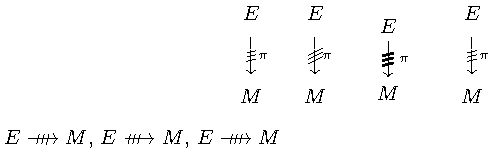
\includegraphics{full-examples/ex-setup-out.pdf}}\end{center}
\end{minipage}\par\medskip
プリアンブルの\verb|\folarrowsetup{gap=0.45}|は文書全体に効く．グループ（\verb|{|と\verb|}|）の中で使った
\verb|\folarrowsetup|はそのグループの中だけに効き，グループを出ると文書全体の設定に戻る．
図式は左から，文書全体の設定（\verb|gap=0.45|），それに加えて\verb|span=1.5, lean=0.5|，
\verb|thickness=0.8pt|（\pkg{tikz-cd}），文書全体の設定に戻ったもの．本文の数式は左から，文書全体の設定，
それに加えて\verb|shift=0.5|（3本線を矢印の根元の側へずらす），文書全体の設定に戻ったもの．
形のキーが既定値でないので，この例の本文用の矢印は，\ref{sec:glyphs}節の矢印のフォントではなく，
矢印に3本線を描いて組まれる．

斜線の大きさの基準になる矢頭の幅と，線の太さの決め方は\ref{sec:metrics}節で述べる．
\pkg{tikz-cd}では，\verb|thickness|が空なら矢印の軸と同じ太さで描く．

斜線の向きは「$\pm\text{lean}\times$矢印の向き＋法線」の2通りのうち，右上がりになるほうを選ぶ．
横向きの矢印では立った「///」，縦向きの矢印では右上がりのほぼ水平な3本になる．

\section{矢頭の幅と線の太さ}\label{sec:metrics}

斜線の長さ・間隔は矢頭の幅を，線の太さは矢印の軸の太さを基準にする．
これらはフォントによって大きく異なり（同じ10\,ptでも矢頭の幅は2.4\,ptから5.6\,ptまである），
フォントの寸法情報（TFMや\verb|\fontdimen|）からは正しく求められないことが多い．
そこで，その場で使われている矢印のフォントについて，次の順に求める．
\begin{enumerate}
\item \textbf{Lua\LaTeX＋OpenTypeの数式フォント}：矢印の箱の中のグリフの外接矩形をフォントから直接読み，
  矢頭の幅とする．線の太さは同じフォントのマイナス記号（U+2212）の高さとする．
  添字の大きさで使われる添字用の字形（OpenTypeのssty）や，\verb|\Big|の大きい字形も読む
  （\file{folarrow.lua}）．
\item \textbf{Xe\LaTeX＋OpenTypeの数式フォント}：\verb|\XeTeXglyphbounds|でグリフの外接矩形を読む．
  添字用の字形と\verb|\Big|の大きい字形は読めないので，元の字形の値になる．
\item \textbf{Type 1の数式フォント}（pdf\LaTeX，up\LaTeX，Lua\LaTeX）：実測データ（\file{folarrow-fonts.def}）を引く．
  矢印の文字を持つフォントは，\verb|\rightarrow|の数式文字コードと\verb|\downarrow|の区切り記号コードから求める
  （\pkg{drm}や\pkg{euler}のように，矢印を記号フォント以外から取るパッケージがあるため）．
  データはフォント名（\verb|\fontname|の基本部分）ごとに，矢頭の幅と軸の太さのquadに対する比を持つ．
  cmsy7とcmsy10のように光学サイズで形が違うものは，それぞれの名前で持つ．
\item \textbf{どれにも当たらないとき}：\verb|\rightarrow|の箱の高さと数式の軸の高さ，数式拡張フォントの
  罫線の太さから推定する．極端な値にならないよう，quadに対する比を制限する．
\end{enumerate}
マイナス記号の太さが矢印の軸と異なるOpenTypeフォント（Asana Math，GFS Neohellenic Math，
Minion Mathの\verb|\Big|の字形，KpMathの\verb|\Big|の字形）には，実測による補正を掛ける．

\subsection{3本線の位置}

3本線は矢印の字面の中心（軸の上の，矢印の長さの中央）に置く．矢印の箱の中心と字面の中心は
一致しないことが多い（\verb|\foldownarrow|，\verb|\foluparrow|の土台や\verb|\longrightarrow|では，
矢頭の側へ0.1～0.7\,ptほどずれ，書体によっては軸に直交する方向にも0.1～0.3\,ptずれる）．
左向きの矢印は右向きの矢印を左右反転した形とは限らないので，ずれ方も右向きと同じではない．
そこで，8種類の矢印（\verb|\longrightarrow|，\verb|\longleftarrow|，右向き・左向きの伸びる矢印，
\verb|\Big|の下向き・上向き，\verb|\foldownarrow|・\verb|\foluparrow|の土台）のそれぞれについて，
矢印の向きと直交方向の2方向で箱の中心と字面の中心の差を実測データに持ち，3本線をその分だけ動かす．
Lua\LaTeX{}とXe\LaTeX{}では，横向きの矢印の3本線の高さを，グリフの外接矩形から求めた矢頭の上下の中心にする．

\verb|\foldownarrow|，\verb|\foluparrow|の土台は，記号フォントのquadの1.25倍の高さの区切り記号で組む．
\verb|\right.|が足す空の区切り記号の幅（\verb|\nulldelimiterspace|）は0にし，区切り記号の字形の選び方が
文字の大きさや本文のフォントによらないよう，\verb|\delimiterfactor|を1000，\verb|\delimitershortfall|を0にする．

伸びる矢印（\pkg{amscd}の横矢印，\verb|\xfolrightarrow|）では，軸をつなぐ\verb|\cleaders|の割り付けが
矢印の長さによって変わるため，書体によっては0.1\,ptほどのずれが残る（STIXで0.14\,pt，\pkg{pxfonts}のボールドで0.17\,pt）．

\ref{sec:glyphs}節の矢印のフォントでは，3本線を字形の輪郭から求めた字面の中央に置いて字形にしている．
10\,ptのComputer Modern，\pkg{newtxmath}，\pkg{newpxmath}，\pkg{txfonts}の4方向の矢印を2400\,dpiで
画像にして測ると，矢印の向きと直交方向のどちらでも，中央からのずれは0.015\,pt以下（画素の半分）だった．
OpenTypeの数式フォント用のOTFでは，XITS Math Bold以外の48書体をLua\LaTeX{}とXe\LaTeX{}で組み，4方向の矢印を同じように測った．
直交方向のずれは全書体で0.03\,pt以下，矢印の向きのずれは，Pennstander Mathの9つとLuciole Math Boldを除いて
0.03\,pt以下だった．この10書体は矢頭の返しが長く後ろへ伸びていて，画像での測り方（矢印の長さの25〜75\%の範囲で
3本線を探す）に矢頭が入り込むため，画像では測れない．そこで，全書体の字形について，字形から元の矢印を
差し引いて3本線だけを取り出し，その中心を輪郭の座標で比べたところ，ずれは0.0002\,em以下（座標を整数に
丸めた誤差）だった．

Pennstander Mathの太いウェイト（Bold以上）では，軸の太さが3本線の間隔とほぼ同じになるので，3本線が
つながって見える（形の規則どおりの結果である）．
Luciole MathはLua\LaTeX{}で，↑の伸びる区切り記号が「Extensible recipe has no fixed parts」のエラーになる
（フォントの問題で，\pkg{folarrow}を使わなくても起きる）．OTFの字形で組む場合はこの区切り記号を使わないので
影響しないが，\verb|glyphs=false|などで描く場合（つねに描く簡易版\verb|lite|を含む）の\verb|\foluparrow|は
このエラーになる．

\subsection{3本線の端の形}

3本線の端は，矢印の尻（軸の端）の形に合わせる．尻が丸い矢印では丸い端，
そうでない矢印では切りっぱなしにする．丸い端は線の太さの半分だけ外にはみ出すので，
見た目の長さがそろうよう，そのぶん短く引く．
\begin{itemize}
\item \pkg{amscd}，本文の数式：実際に使う矢印の組み方（\verb|\longrightarrow|，伸びる矢印，
  \verb|\Big\downarrow|，\verb|\foldownarrow|の土台）ごとに，尻の形を実測データに持つ．
  たとえばComputer Modernでは，横向きの矢印は尻が丸く（\verb|\relbar|の端が丸い），
  \verb|\Big\downarrow|は上端が平らなので，横向きは丸い端，縦向きは切りっぱなしになる．
  OpenTypeの数式フォントはフォント名で表を引く（Latin Modern Math，New Computer Modern Mathは丸，
  ほかは切りっぱなし）．表にないフォントでは切りっぱなしにする．
\item \pkg{xy-pic}：\pkg{xy-pic}の線の端は丸いので，丸い端にする．
\item \pkg{tikz-cd}：矢印の線の端の設定（\verb|line cap|）をそのまま使う．\pkg{tikz-cd}の既定は切りっぱなしである．
\end{itemize}

\subsection{検証}

\LaTeX{} Font Catalogueの「Fonts with Math Support」（\url{https://tug.org/FontCatalogue/mathfonts.html}）の全書体（68）と，
OpenTypeの数式フォント（Latin Modern Math，New Computer Modern Math，STIX Two Math，
\TeX{} Gyre Termes／Pagella／Bonum／Schola／DejaVu Math，Libertinus Math，Fira Math，XITS Math，
Asana Math，Erewhon Math，KpMath，GFS Neohellenic Math，Minion Math），および
Computer Modern，Latin Modern，\pkg{newtx}，\pkg{txfonts}，\pkg{newpx}，\pkg{pxfonts}のボールド（\verb|\boldmath|）について，
矢印を実際に組んで2400\,dpiの画像にし，字面の範囲を測って\pkg{folarrow}の計算値と比べた．
大きさは10\,pt，10.95\,pt，12\,pt，スタイルは本文・添字・添字の添字，縦向きは\verb|\Big\downarrow|と
\verb|\foldownarrow|の土台である．エンジンはType 1系をpdf\LaTeX{}とup\LaTeX，OpenType系をLua\LaTeX{}とXe\LaTeX{}で組んだ．

次の表は計算値と実測値のずれの最大（\%）で，3\%を超えるものを太字にした．
「中心」の欄は，3本線の中心と矢印の字面の中心のずれの最大（pt，矢印の向きと直交方向，8種類の矢印の
すべての大きさにわたる）で，0.05\,ptを超えるものを太字にした．
「端」の欄は，実測した矢印の尻の形（丸か平らか）と\pkg{folarrow}が選ぶ3本線の端の形が，
4種類の矢印（\verb|\longrightarrow|，伸びる矢印，\verb|\Big\downarrow|，\verb|\foldownarrow|の土台）の
すべてで一致すれば○とした．
3\%を超えるのは次のものだけである．
\begin{itemize}
\item \textbf{PKフォント}（\pkg{boisik}，Computer Concrete，\pkg{drm}）：METAFONTのビットマップフォントで，
  ドットの段差（600\,dpiで0.12\,pt）がそのまま寸法の誤差になる．フォント自体の性質である．
\item \textbf{添字用字形}（Xe\LaTeX{}のSTIX Two Math，Erewhon Math）：Xe\TeX{}では添字用の字形を
  読めないため，添字の大きさで最大20\%ずれる．Lua\LaTeX{}では正しく求まる．
\item \textbf{未インストール}：URW Garamond（\pkg{mathdesign}）と\pkg{garamondx}は非フリーのフォントで，
  検証した環境（\TeX{} Live 2026）に入っていないため確認していない．
\end{itemize}
表とデータは，矢印を実際に組んで測った結果から作成した．

{\small% folarrow-verify.tex：矢印を実際に組んで測った結果から作成した検証表（手で直さない）
\begin{longtable}{@{}lcrrrrrcl@{}}
書体（設定） & エンジン & \multicolumn{2}{c}{横向き} & \multicolumn{2}{c}{縦向き} & 中心 & 端 & 備考\\
 & & 幅 & 太さ & 幅 & 太さ & pt & & \\\hline\endhead
\texttt{antykwatorunska} & pdf & 1 & 0 & 0 & 0 & 0.05 & ○ & \\
\texttt{antykwatorunska} & up & 1 & 0 & 0 & 0 & \textbf{0.06} & ○ & \\
\texttt{antykwatorunskacondensed} & pdf & 1 & 0 & 0 & 0 & 0.02 & ○ & \\
\texttt{antykwatorunskacondensed} & up & 1 & 0 & 0 & 0 & 0.02 & ○ & \\
\texttt{antykwatorunskalight} & pdf & 1 & 0 & 0 & 0 & \textbf{0.07} & ○ & \\
\texttt{antykwatorunskalight} & up & 1 & 0 & 0 & 0 & \textbf{0.07} & ○ & \\
\texttt{antykwatorunskalightcondensed} & pdf & 1 & 0 & 0 & 0 & 0.02 & ○ & \\
\texttt{antykwatorunskalightcondensed} & up & 1 & 0 & 0 & 0 & 0.03 & ○ & \\
\texttt{arev} & pdf & 1 & 0 & 0 & 0 & 0.03 & ○ & \\
\texttt{arev} & up & 1 & 0 & 0 & 0 & 0.05 & ○ & \\
\texttt{Asana-Math.otf} & Lua & 1 & 0 & 1 & 0 & 0.03 & ○ & \\
\texttt{Asana-Math.otf} & Xe & 1 & 0 & 1 & 0 & 0.03 & ○ & \\
\texttt{asanamath} & Lua & 1 & 0 & 1 & 0 & 0.03 & ○ & \\
\texttt{baskervaldx} & pdf & 0 & 0 & 0 & 0 & 0.02 & ○ & \\
\texttt{baskervaldx} & up & 0 & 0 & 0 & 0 & 0.02 & ○ & \\
\texttt{baskervillef} & pdf & 0 & 0 & 0 & 0 & 0.02 & ○ & \\
\texttt{baskervillef} & up & 0 & 0 & 0 & 0 & 0.02 & ○ & \\
\texttt{boisik} & pdf & \textbf{12} & \textbf{27} & 0 & 0 & \textbf{0.20} & ○ & PKフォント\\
\texttt{boisik} & up & \textbf{12} & \textbf{27} & 0 & 0 & \textbf{0.29} & ○ & PKフォント\\
\texttt{charterbt} & pdf & 2 & 0 & 0 & 0 & 0.02 & ○ & \\
\texttt{charterbt} & up & 2 & 0 & 0 & 0 & \textbf{0.05} & ○ & \\
\texttt{cochineal} & pdf & 0 & 0 & 0 & 0 & 0.02 & ○ & \\
\texttt{computerconcrete} & pdf & 1 & \textbf{10} & 0 & 0 & 0.05 & ○ & PKフォント\\
\texttt{computerconcrete} & up & 1 & \textbf{10} & 0 & 0 & \textbf{0.14} & ○ & PKフォント\\
\texttt{computerconcreteeuler} & pdf & 0 & 0 & 0 & 0 & 0.03 & ○ & \\
\texttt{computerconcreteeuler} & up & 0 & 0 & 0 & 0 & 0.04 & ○ & \\
\texttt{computermodern} & pdf & 0 & 0 & 0 & 0 & 0.03 & ○ & \\
\texttt{computermodern} & up & 0 & 0 & 0 & 0 & 0.04 & ○ & \\
\texttt{computermodern-bold} & pdf & 0 & 0 & 0 & 0 & 0.03 & ○ & \\
\texttt{computermodern-bold} & up & 0 & 0 & 0 & 0 & 0.03 & ○ & \\
\texttt{computermodernbright} & pdf & 0 & 0 & 0 & 0 & 0.02 & ○ & \\
\texttt{computermodernbright} & up & 0 & 0 & 0 & 0 & 0.03 & ○ & \\
\texttt{domitian} & pdf & 1 & 0 & 0 & 0 & 0.02 & ○ & \\
\texttt{domitian} & up & 1 & 0 & 0 & 0 & 0.04 & ○ & \\
\texttt{drm} & pdf & \textbf{3} & \textbf{13} & 0 & \textbf{6} & \textbf{0.47} & ○ & PKフォント\\
\texttt{drm} & up & 0 & \textbf{5} & 0 & \textbf{6} & \textbf{0.47} & ○ & PKフォント\\
\texttt{ebgaramond} & pdf & 0 & 0 & 0 & 0 & 0.02 & ○ & \\
\texttt{ebgaramond} & up & 0 & 0 & 0 & 0 & 0.02 & ○ & \\
\texttt{erewhon} & pdf & 0 & 0 & 0 & 0 & 0.02 & ○ & \\
\texttt{erewhon} & up & 0 & 0 & 0 & 0 & 0.02 & ○ & \\
\texttt{erewhon-math} & Lua & 2 & 0 & 1 & 0 & 0.03 & ○ & \\
\texttt{Erewhon-Math.otf} & Lua & 2 & 0 & 1 & 0 & 0.03 & ○ & \\
\texttt{Erewhon-Math.otf} & Xe & \textbf{6} & \textbf{18} & 1 & 0 & 0.03 & ○ & 添字用字形\\
\texttt{eulervm} & pdf & 0 & 0 & 0 & 0 & 0.02 & ○ & \\
\texttt{europeancomputerconcrete} & pdf & 1 & \textbf{10} & 0 & 0 & 0.05 & ○ & PKフォント\\
\texttt{europeancomputerconcrete} & up & 1 & \textbf{10} & 0 & 0 & \textbf{0.14} & ○ & PKフォント\\
\texttt{europeancomputerconcreteeuler} & pdf & 0 & 0 & 0 & 0 & 0.03 & ○ & \\
\texttt{europeancomputerconcreteeuler} & up & 0 & 0 & 0 & 0 & 0.04 & ○ & \\
\texttt{europeancomputermodern} & pdf & 0 & 0 & 0 & 0 & 0.03 & ○ & \\
\texttt{europeancomputermodern} & up & 0 & 0 & 0 & 0 & 0.04 & ○ & \\
\texttt{europeancomputermodernbright} & pdf & 0 & 0 & 0 & 0 & 0.02 & ○ & \\
\texttt{europeancomputermodernbright} & up & 0 & 0 & 0 & 0 & 0.03 & ○ & \\
\texttt{Fira Math} & Lua & 2 & 0 & 1 & 0 & 0.02 & ○ & \\
\texttt{FiraMath-Regular.otf} & Lua & 2 & 0 & 1 & 0 & 0.02 & ○ & \\
\texttt{FiraMath-Regular.otf} & Xe & 2 & 0 & 1 & 0 & 0.02 & ○ & \\
\texttt{firasansmath} & Lua & 2 & 0 & 1 & 0 & 0.02 & ○ & \\
\texttt{firasansnewtxsf} & pdf & 0 & 0 & 0 & 0 & 0.02 & ○ & \\
\texttt{firasansnewtxsf} & up & 0 & 0 & 0 & 0 & 0.02 & ○ & \\
\texttt{fourier-only} & pdf & 1 & 0 & 0 & 0 & 0.04 & ○ & \\
\texttt{garamond} & pdf & -- & -- & -- & -- & -- & -- & 未インストール\\
\texttt{garamond} & up & -- & -- & -- & -- & -- & ○ & 未インストール\\
\texttt{garamondexpertmathdesign} & pdf & -- & -- & -- & -- & -- & -- & 未インストール\\
\texttt{garamondexpertmathdesign} & up & -- & -- & -- & -- & -- & -- & 未インストール\\
\texttt{garamondexpertnewtxmath} & pdf & -- & -- & -- & -- & -- & -- & 未インストール\\
\texttt{garamondexpertnewtxmath} & up & -- & -- & -- & -- & -- & -- & 未インストール\\
\texttt{gfsartemisia} & pdf & 1 & 0 & 0 & 0 & 0.03 & ○ & \\
\texttt{gfsartemisia} & up & 1 & 0 & 0 & 0 & 0.02 & ○ & \\
\texttt{gfsartemisiaeulermath} & pdf & 0 & 0 & 0 & 0 & 0.03 & ○ & \\
\texttt{gfsartemisiaeulermath} & up & 0 & 0 & 0 & 0 & 0.04 & ○ & \\
\texttt{gfsneohellenic} & pdf & 0 & 0 & 0 & 0 & 0.03 & ○ & \\
\texttt{gfsneohellenic} & up & 0 & 0 & 0 & 0 & 0.04 & ○ & \\
\texttt{gfsneohellenicmath} & Lua & 1 & 2 & 1 & 0 & 0.04 & ○ & \\
\texttt{GFSNeohellenicMath.otf} & Lua & 1 & 2 & 1 & 0 & 0.03 & ○ & \\
\texttt{GFSNeohellenicMath.otf} & Xe & 1 & 2 & 1 & 0 & 0.03 & ○ & \\
\texttt{heuristica} & pdf & 0 & 0 & 0 & 0 & 0.02 & ○ & \\
\texttt{heuristica} & up & 0 & 0 & 0 & 0 & 0.02 & ○ & \\
\texttt{iwona} & pdf & 1 & 0 & 0 & 0 & 0.03 & ○ & \\
\texttt{iwona} & up & 1 & 0 & 0 & 0 & 0.03 & ○ & \\
\texttt{iwonacondensed} & pdf & 1 & 0 & 0 & 0 & 0.03 & ○ & \\
\texttt{iwonacondensed} & up & 1 & 0 & 0 & 0 & 0.02 & ○ & \\
\texttt{iwonalight} & pdf & 1 & 0 & 0 & 0 & 0.02 & ○ & \\
\texttt{iwonalight} & up & 1 & 0 & 0 & 0 & 0.02 & ○ & \\
\texttt{iwonalightcondensed} & pdf & 1 & 0 & 0 & 0 & 0.02 & ○ & \\
\texttt{iwonalightcondensed} & up & 1 & 0 & 0 & 0 & 0.02 & ○ & \\
\texttt{kerkis} & pdf & 1 & 0 & 0 & 0 & 0.03 & ○ & \\
\texttt{kerkis} & up & 1 & 0 & 0 & 0 & 0.02 & ○ & \\
\texttt{KpMath-Regular.otf} & Lua & 2 & 0 & 1 & 1 & 0.02 & ○ & \\
\texttt{KpMath-Regular.otf} & Xe & 2 & 0 & 0 & 1 & 0.02 & ○ & \\
\texttt{kpsansserif} & pdf & 0 & 0 & 0 & 0 & 0.04 & ○ & \\
\texttt{kpsansserif} & up & 0 & 0 & 0 & 0 & 0.05 & ○ & \\
\texttt{kpserif} & pdf & 0 & 0 & 0 & 0 & 0.04 & ○ & \\
\texttt{kpserif} & up & 0 & 0 & 0 & 0 & 0.05 & ○ & \\
\texttt{kurier} & pdf & 1 & 0 & 0 & 0 & 0.03 & ○ & \\
\texttt{kurier} & up & 1 & 0 & 0 & 0 & 0.03 & ○ & \\
\texttt{kuriercondensed} & pdf & 1 & 0 & 0 & 0 & 0.03 & ○ & \\
\texttt{kuriercondensed} & up & 1 & 0 & 0 & 0 & 0.02 & ○ & \\
\texttt{kurierlight} & pdf & 1 & 0 & 0 & 0 & 0.02 & ○ & \\
\texttt{kurierlight} & up & 1 & 0 & 0 & 0 & 0.02 & ○ & \\
\texttt{kurierlightcondensed} & pdf & 1 & 0 & 0 & 0 & 0.02 & ○ & \\
\texttt{kurierlightcondensed} & up & 1 & 0 & 0 & 0 & 0.02 & ○ & \\
\texttt{Latin Modern Math} & Lua & 1 & 0 & 1 & 0 & 0.02 & ○ & \\
\texttt{latinmodern-math.otf} & Lua & 1 & 0 & 1 & 0 & 0.02 & ○ & \\
\texttt{latinmodern-math.otf} & Lua & 1 & 0 & 1 & 0 & 0.02 & ○ & \\
\texttt{latinmodern-math.otf} & Xe & 1 & 0 & 0 & 0 & 0.02 & ○ & \\
\texttt{latinmodernroman} & pdf & 0 & 0 & 0 & 0 & 0.03 & ○ & \\
\texttt{latinmodernroman} & up & 0 & 0 & 0 & 0 & 0.02 & ○ & \\
\texttt{latinmodernroman-bold} & pdf & 0 & 0 & 0 & 0 & 0.02 & ○ & \\
\texttt{latinmodernroman-bold} & up & 0 & 0 & 0 & 0 & 0.03 & ○ & \\
\texttt{Libertinus Math} & Lua & 1 & 0 & 1 & 0 & 0.01 & ○ & \\
\texttt{LibertinusMath-Regular.otf} & Lua & 1 & 0 & 1 & 0 & 0.01 & ○ & \\
\texttt{LibertinusMath-Regular.otf} & Xe & 1 & 0 & 1 & 0 & 0.02 & ○ & \\
\texttt{libertinusserif} & pdf & 0 & 0 & 0 & 0 & 0.03 & ○ & \\
\texttt{libertinusserif} & up & 0 & 0 & 0 & 0 & 0.04 & ○ & \\
\texttt{linuxlibertine} & pdf & 0 & 0 & 0 & 0 & 0.02 & ○ & \\
\texttt{linuxlibertine} & up & 0 & 0 & 0 & 0 & 0.02 & ○ & \\
\texttt{lxfonts} & pdf & 0 & 0 & 0 & 0 & 0.02 & ○ & \\
\texttt{lxfonts} & up & 0 & 0 & 0 & 0 & 0.03 & ○ & \\
\texttt{Minion Math} & Lua & 1 & 0 & 1 & 0 & 0.02 & ○ & \\
\texttt{Minion Math} & Lua & 1 & 0 & 1 & 0 & 0.02 & ○ & \\
\texttt{Minion Math} & Xe & 1 & 0 & 1 & 0 & 0.02 & ○ & \\
\texttt{mlmodern} & pdf & 0 & 0 & 0 & 0 & 0.03 & ○ & \\
\texttt{mlmodern} & up & 0 & 0 & 0 & 0 & 0.04 & ○ & \\
\texttt{NewCMMath-Regular.otf} & Lua & 1 & 0 & 1 & 0 & 0.02 & ○ & \\
\texttt{NewCMMath-Regular.otf} & Xe & 1 & 0 & 0 & 0 & 0.02 & ○ & \\
\texttt{newcomputermodernroman} & Lua & 1 & 0 & 1 & 0 & 0.02 & ○ & \\
\texttt{newpx} & pdf & 1 & 0 & 0 & 0 & 0.03 & ○ & \\
\texttt{newpx} & up & 1 & 0 & 0 & 0 & 0.03 & ○ & \\
\texttt{newpx-bold} & pdf & 1 & 0 & 0 & 0 & \textbf{0.07} & ○ & \\
\texttt{newpx-bold} & up & 1 & 0 & 0 & 0 & \textbf{0.07} & ○ & \\
\texttt{newpxeuler} & pdf & 1 & 0 & 0 & 0 & 0.03 & ○ & \\
\texttt{newpxeuler} & up & 1 & 0 & 0 & 0 & 0.03 & ○ & \\
\texttt{newtx} & pdf & 0 & 0 & 0 & 0 & 0.02 & ○ & \\
\texttt{newtx} & up & 0 & 0 & 0 & 0 & 0.02 & ○ & \\
\texttt{newtx-bold} & pdf & 0 & 0 & 0 & 0 & 0.04 & ○ & \\
\texttt{newtx-bold} & up & 0 & 0 & 0 & 0 & \textbf{0.06} & ○ & \\
\texttt{newtxsf} & pdf & 0 & 0 & 0 & 0 & 0.02 & ○ & \\
\texttt{notoserif} & pdf & 0 & 0 & 0 & 0 & 0.02 & ○ & \\
\texttt{notoserif} & up & 0 & 0 & 0 & 0 & 0.02 & ○ & \\
\texttt{pxfonts} & pdf & 0 & 0 & 0 & 0 & 0.02 & ○ & \\
\texttt{pxfonts} & up & 0 & 0 & 0 & 0 & 0.02 & ○ & \\
\texttt{pxfonts-bold} & pdf & 1 & 0 & 0 & 0 & \textbf{0.17} & ○ & \\
\texttt{pxfonts-bold} & up & 1 & 0 & 0 & 0 & \textbf{0.09} & ○ & \\
\texttt{sansmathfonts} & pdf & 0 & 0 & 0 & 0 & 0.02 & ○ & \\
\texttt{sansmathfonts} & up & 0 & 0 & 0 & 0 & 0.02 & ○ & \\
\texttt{scholax} & pdf & 1 & 0 & 1 & 0 & 0.04 & ○ & \\
\texttt{scholax} & up & 1 & 0 & 1 & 0 & 0.03 & ○ & \\
\texttt{step} & pdf & 1 & 0 & 0 & 0 & \textbf{0.14} & ○ & \\
\texttt{step} & up & 1 & 0 & 0 & 0 & \textbf{0.14} & ○ & \\
\texttt{stickstoo} & pdf & 1 & 0 & 0 & 0 & 0.02 & ○ & \\
\texttt{stickstoo} & up & 1 & 0 & 0 & 0 & 0.02 & ○ & \\
\texttt{stix} & pdf & 1 & 0 & 0 & 0 & \textbf{0.14} & ○ & \\
\texttt{stix} & up & 1 & 0 & 0 & 0 & \textbf{0.14} & ○ & \\
\texttt{STIX Two Math} & Lua & 1 & 2 & 1 & 1 & 0.02 & ○ & \\
\texttt{stix2} & pdf & 1 & 0 & 1 & 1 & 0.02 & ○ & \\
\texttt{stix2} & up & 1 & 0 & 1 & 1 & 0.02 & ○ & \\
\texttt{STIXTwoMath-Regular.otf} & Lua & 1 & 2 & 1 & 1 & 0.02 & ○ & \\
\texttt{STIXTwoMath-Regular.otf} & Xe & \textbf{11} & \textbf{20} & 1 & 1 & 0.02 & ○ & 添字用字形\\
\texttt{TeX Gyre Bonum Math} & Lua & 2 & 0 & 1 & 0 & 0.02 & ○ & \\
\texttt{TeX Gyre DejaVu Math} & Lua & 0 & 0 & 0 & 0 & \textbf{0.06} & ○ & \\
\texttt{TeX Gyre Pagella Math} & Lua & 1 & 0 & 1 & 0 & \textbf{0.06} & ○ & \\
\texttt{TeX Gyre Schola Math} & Lua & 2 & 0 & 1 & 0 & 0.02 & ○ & \\
\texttt{TeX Gyre Termes Math} & Lua & 1 & 0 & 0 & 0 & 0.03 & ○ & \\
\texttt{texgyrebonum-math.otf} & Lua & 2 & 0 & 1 & 0 & 0.02 & ○ & \\
\texttt{texgyrebonum-math.otf} & Xe & 1 & 0 & 1 & 0 & 0.03 & ○ & \\
\texttt{texgyredejavu-math.otf} & Lua & 0 & 0 & 0 & 0 & \textbf{0.06} & ○ & \\
\texttt{texgyredejavu-math.otf} & Xe & 0 & 0 & 0 & 0 & 0.05 & ○ & \\
\texttt{texgyrepagella-math.otf} & Lua & 1 & 0 & 1 & 0 & \textbf{0.06} & ○ & \\
\texttt{texgyrepagella-math.otf} & Xe & 1 & 0 & 1 & 0 & \textbf{0.07} & ○ & \\
\texttt{texgyreschola-math.otf} & Lua & 2 & 0 & 1 & 0 & 0.02 & ○ & \\
\texttt{texgyreschola-math.otf} & Xe & 2 & 0 & 1 & 0 & 0.02 & ○ & \\
\texttt{texgyretermes-math.otf} & Lua & 1 & 0 & 0 & 0 & 0.03 & ○ & \\
\texttt{texgyretermes-math.otf} & Xe & 1 & 0 & 0 & 0 & 0.02 & ○ & \\
\texttt{txfonts} & pdf & 1 & 0 & 0 & 0 & 0.03 & ○ & \\
\texttt{txfonts} & up & 1 & 0 & 0 & 0 & 0.02 & ○ & \\
\texttt{txfonts-bold} & pdf & 1 & 0 & 0 & 0 & 0.04 & ○ & \\
\texttt{txfonts-bold} & up & 1 & 0 & 0 & 0 & 0.04 & ○ & \\
\texttt{urwnimbusroman} & pdf & 0 & 0 & 0 & 0 & 0.02 & ○ & \\
\texttt{urwnimbusroman} & up & 0 & 0 & 0 & 0 & 0.03 & ○ & \\
\texttt{urwpalladio} & pdf & 1 & 0 & 0 & 0 & 0.02 & ○ & \\
\texttt{urwpalladio} & up & 1 & 0 & 0 & 0 & 0.02 & ○ & \\
\texttt{urwschoolbookl} & pdf & 1 & 0 & 0 & 0 & 0.04 & ○ & \\
\texttt{urwschoolbookl} & up & 1 & 0 & 0 & 0 & \textbf{0.06} & ○ & \\
\texttt{utopia-fouriermath} & pdf & 1 & 0 & 0 & 0 & 0.04 & ○ & \\
\texttt{utopia-fouriermath} & up & 1 & 0 & 0 & 0 & \textbf{0.06} & ○ & \\
\texttt{utopia-mathdesign} & pdf & 2 & 0 & 0 & 0 & 0.02 & ○ & \\
\texttt{utopia-mathdesign} & up & 2 & 0 & 0 & 0 & \textbf{0.05} & ○ & \\
\texttt{xits} & Lua & 1 & 0 & 1 & 0 & 0.02 & ○ & \\
\texttt{XITS Math} & Lua & 1 & 0 & 1 & 0 & 0.02 & ○ & \\
\texttt{XITSMath-Regular.otf} & Lua & 1 & 0 & 1 & 0 & 0.02 & ○ & \\
\texttt{XITSMath-Regular.otf} & Xe & 1 & 0 & 1 & 1 & 0.02 & ○ & \\
\end{longtable}
}

\section{動作環境}

pdf\LaTeX，Lua\LaTeX，up\LaTeX＋dvipdfmx，Xe\LaTeX{}で動作を確認した（\TeX{} Live 2025と2026）．
LaTeXの2022-06-01以降が必要である（\verb|\fpeval|と\verb|\DeclareKeys|を使うため）．
ただしTeX Live 2025と2026のLua\LaTeX{}では\pkg{xy-pic}自体がxypdfのエラーで使えない（\pkg{folarrow}とは無関係）．

\section{使うときの注意}\label{sec:notes}

\begin{itemize}
\item \textbf{キーの値}：数でない値や範囲の外の値（\ref{sec:shape}節の表）を与えると，キーの名前と値を示す
  エラーになり，前の値のままになる．
\item \textbf{見出しと目次}：\verb|\section|，\verb|\caption|などの引数でも使える（頑健な命令である）．
  \pkg{hyperref}のしおりでは，本文用の矢印は→←↓↑の文字に，伸びる矢印はラベルを除いた→←になる．
\item \textbf{読み込み順}：\pkg{amscd}，\pkg{xy-pic}，\pkg{tikz-cd}，\pkg{unicode-math}は，\pkg{folarrow}の前後
  どちらで読み込んでもよい．
\item \textbf{dvips}：dvipsはパッケージからマップファイルを読ませられないので，\file{folarrow.map}を登録する
  （\verb|updmap-user --enable Map=folarrow.map|，一時的には\verb|dvips -u +folarrow.map|）．登録しないと，
  本文用の矢印がほかの文字（Computer Modernでは$\Gamma\Delta\Theta\Lambda$）に置き換わる．dvipsを使う文書では，
  そのことを知らせる警告を出す．矢印のフォントを使わないなら\verb|glyphs=false|を指定する．
\item \textbf{日本語の組版}：pLaTeX，upLaTeX，Lua\TeX-ja（\pkg{unicode-math}と一緒に使う場合を含む），
  Xe\LaTeX{}＋\pkg{xeCJK}で使える．pTeX／upTeX＋dvipdfmxの縦組みでは，描いて組む3本線を縦組みに合わせて回す．
  縦組みの中で\pkg{tikz-cd}などの図式を組むときは，\verb|\hbox{\yoko …}|などで横組みの箱に入れる
  （縦のままの\pkg{tikz-cd}は，Ti\textit{k}Z自体が崩れる）．
\item \textbf{babel}：spanishでは\verb|<|と\verb|>|が能動文字になり，\pkg{amscd}そのものが使えなくなる
  （\pkg{folarrow}を使わなくても起きる）．\verb|es-noquoting|オプションか\verb|\deactivatequoting|を使えば，
  \verb|@F>>>|なども使える．german，russianなどで\pkg{tikz-cd}を使うときは，\verb|\usetikzlibrary{babel}|が要る
  （\pkg{tikz-cd}の制限）．
\item \textbf{色}：\verb|\color|の中の矢印と，\pkg{tikz-cd}で色を付けた矢印では，3本線も同じ色になる．
  \pkg{xy-pic}の\verb|\ar@[red]|は\verb/|@{fol}/に色を引き継がない（\verb/|@{>}/などと同じ\pkg{xy-pic}の仕様）ので，
  \verb/\ar@[red][r]|*[red]\dir{fol}/のように書く．
\item \textbf{\pkg{tikz-cd}の線の種類}：\verb|dashed|，\verb|dotted|の矢印でも，3本線は実線で描く．
\item \textbf{大きな文字}：描いて組む縦向きの矢印と\pkg{amscd}の縦向きの矢印は大きな区切り記号で組むので，
  大きな文字ではexscale（\pkg{amsmath}が読み込む）がないと矢印が小さいままになる．\pkg{amsmath}かexscaleを
  読み込むとよい．\pkg{amscd}の横向きの矢印は，\verb|\longrightarrow|の長さより短くしない（大きな文字で
  \verb|\minCDarrowwidth|の2.5\,pcが短すぎて3本線が矢頭にかかるのを避ける）．
\item \textbf{短い矢印}：\verb|\minCDarrowwidth|を小さくしたり，\pkg{tikz-cd}の\verb|column sep=tiny|，
  \pkg{xy-pic}の\verb|@C=0.5pc|などで矢印をとても短くしたりすると，3本線が矢印からはみ出して見える．
\item \textbf{タグ付けしたPDF}：\verb|\DocumentMetadata{tagging=on}|などでは，描いた3本線は図ではなく
  飾り（artifact）として扱う．
\item \textbf{処理時間}：本文用の矢印をフォントの字形で組む場合（既定）は，\pkg{folarrow}を使わない場合と
  ほとんど変わらない．描いて組む場合（\verb|glyphs=false|，\verb|lite|，表にない数式フォント）は，
  矢印1つにつき十数ミリ秒かかる．
\end{itemize}

\section{ライセンスと作者}

\file{folarrow.sty}，\file{folarrow.lua}，\file{.def}ファイル，説明書，ツールは，MITライセンス
（\file{LICENSE}）で配布する．矢印のフォント（\file{fonts/}）は元のフォントから作ったもので，元のフォントの
ライセンス（SIL Open Font License 1.1，GUST Font License，フォントの例外付きのGNU GPL）を引き継ぐ．
フォントごとの元のフォント，元の著作権表示，ライセンスは\file{licenses/FONTS.md}にあり，ライセンスの本文も
\file{licenses/}に置いた．

作者：木枝祐介

\end{document}
